\documentclass[../main.tex]{subfiles}
\begin{document}
\chapter{FedRAMP - Federal Risk and Authorization Management Program}
\section{Introduzione}
In questo capitolo verrà approfondito FedRAMP, il programma federale americano per la gestione del rischio e delle autorizzazioni nella cloud.
Sarà proposta un'analisi degli obiettivi del programma, specificando le problematiche in esso affrontate in relazione anche a quanto descritto nel capitolo precedente.
Verrà poi esposta la struttura del documento, dopodiché ci si concentrerà sulla struttura dello stesso approfondendo i ruoli degli attori coinvolti.
In conclusione saranno esposti i concetti di \textit{readiness} e di \textit{compliance} al programma, e sarà approfondito il ruolo dello stesso in Amazon AWS.

\section{Cos'è FedRAMP}
FedRAMP è il programma governativo americano l'applicazione del \textbf{FISMA} (Federal Information Security Management Act) nell'adozione di tecnologie cloud.
Esso propone un approccio standardizzato al \textit{security assessment}, alle autorizzazioni e al monitoraggio continuo di prodotti e servizi cloud, fornendo un insieme di requisiti di sicurezza e un programma di assessment indipendente, nato dalla collaborazione di esperti di sicurezza e di tecnologie cloud.
Le entità coinvolte nella redazione di questo programma sono state molte: la General Services Administration (GSA), il National Institute of Standards and Technology (NIST), il dipartimento di Sicurezza Nazionale (Department of Homeland Security, DHS), il dipartimento della Difesa (Department of Defense, DOD), la National Security Agency (NSA), l'Office of Management and Budget (OMB).

I \textit{cloud service provider} che vogliono offrire servizi per la pubblica amministrazione americana e gli uffici federali devono essere autorizzati tramite questo programma.
Nonostante sia stato sviluppato nel contesto USA, la dinamicità e l'elasticità di FedRAMP ne ha permesso l'adozione \textit{de-facto} anche in altre nazioni, specialmente dell'Asia orientale e del nord Europa.
\subsection{FISMA, Federal Information Security Management Act}
Il FISMA è uno standard di sicurezza, entrato in vigore come legge il 17 Dicembre 2002 come "Titolo III" dell'E-Government Act\cite{united2004information}: ciascun sistema che ospiti dati governativi deve essere autorizzato tramite il FISMA prima di essere messo in produzione.
Esso definisce tre obiettivi principali per la sicurezza dei sistemi informativi federali:
\begin{itemize}
    \item \textbf{Confidenzialità}, per garantire restrizioni autorizzate sull'accesso e la \textit{disclosure} dei dati, con l'obiettivo di proteggere la privacy ed eventuale informazioni sul proprietario odegli stessi
    \item \textbf{Integrità}, per proteggere il dato da manipolazioni o azioni distruttive e per garantire allo stesso tempo l'autenticità e la non-repudiabilità dell'informazione
    \item \textbf{Disponibilità}, per assicurare condizioni di affidabilità nell'accesso al dato
\end{itemize}

A tal fine il \textbf{NIST} ha prodotto il \textbf{Federal Information Risk Management Framework}(\textit{RMF}) il quale organizza i sistemi informatici sulla base del livello di rischio e descrive un insieme minimo di requisiti che devono essere rispettati per garantire un livello di sicurezza adeguato\cite{nist2003nist}, fornendo una metodologia per la selezione dei controlli di sicurezza e per l'esecuzione del deployment e dell'assessment.

\begin{figure}[H]
\centering
\makebox[\textwidth]{
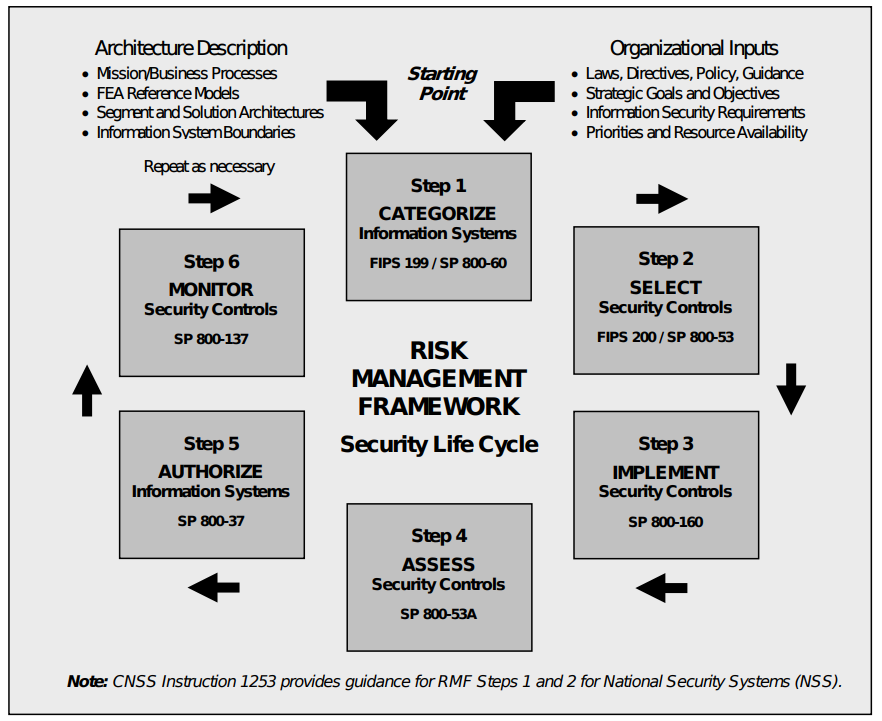
\includegraphics[width=0.8\textwidth]{immagini/risk_management_framework.png}
}
\caption{Risk Management Framework, da \cite{nist2003nist} }\label{fig:riskmanagementfw}
\end{figure}

Tramite la figura \ref{fig:riskmanagementfw} è possibile identificare le sei fasi che compongono il processo di gestione del rischio, ciclico e continuo, identificato dal framework:

\begin{itemize}
    \item \textbf{Categorizzazione del sistema informativo}, tramite i documenti FIPS\footnote{Federal Information Processing Standards} 199 e SP 800-60. Il documento FIPS 199 classifica i sistemi in base al livello di rischio, e contiene i criteri da utilizzare nella categorizzazione. Questi criteri sono basati sull'impatto potenziale di una violazione delle proprietà di confidenzialità, integrità e disponibilità sul sistema e sono: i) Rischio basso, impatto limitato, ii) Rischio medio, con serie conseguenze, iii) Rischio elevato con conseguenze gravi e catrastofiche. FIPS 199 si applica a tutti i sistemi, ad esclusione di quelli designati per l'uso della sicurezza nazionale.
    \item \textbf{Selezione dei controlli di sicurezza}, mediante i documenti FIPS 200 e SP 800-53. FIPS 200 fornisce i requisiti di sicurezza minimi (e i relativi controlli) per ogni categoria definita nel FIPS 199.
        Il documento NIST 800-53 invece definisce i controlli di sicurezza e fornisce le linee guida per scegliere i profili da impiegare per soddisfare i requisiti minimi di sicurezza, in base all'impatto del sistema. I controlli di sicurezza sono divisi in 17 famiglie e vengono divisi in tre classi (controlli di gestione, controlli operazionali e controlli tecnici). 
    \item \textbf{Implementazione dei controlli}, guidata dal documento SP 800-160
    \item \textbf{Assessment dei controlli di sicurezza}, regolato dal documento SP 800-53/A
    \item \textbf{Autorizzazione del sistema informativo}, basata sul documento SP 800-37
    \item \textbf{Fase di monitoraggio}        
\end{itemize}

\subsection{Obiettivo di FedRAMP}
L'obiettivo di FedRAMP è quindi quello di fornire un framework per semplificare il processo di autorizzazione dei servizi cloud adottati dagli enti governativi USA.
Prima dell'adozione di questo programma i produttori di sistemi e applicativi dovevano eseguire l'intero processo di autorizzazione per ciascuna delle agenzie che adottasse il sistema, così come ogni ente gestiva un processo di gestione del rischio a sé stante, anche nel caso in cui un'altra agenzia avesse già adottato servizi e misure di sicurezza analoghi. 
FedRAMP affronta la problematica nei seguenti modi:
\begin{itemize}
    \item Fornendo processi di valutazione della sicurezza e autorizzazione congiunti, basati su una serie di requisiti e controlli standardizzati, sulla base dell'impatto del sistema 
    \item Offrendo un programma di analisi della conformità in grado di produrre
    \item Strutturando un processo di analisi e valutazione della conformità condotto da Organizzazioni di terze parti approvate (3PAO), per valutare costantemente la capacità di un provider di servizi cloud (CSP) di soddisfare requisiti di sicurezza desiderati
    \item Coordinando servizi di monitoraggio continuo
    \item Fornendo pacchetti di autorizzazione composti da servizi cloud già revisionati da una Joint Authorization Board (JAB), composta da esperti di sicurezza provienienti dal DHS, dalla GSA e del DoD. 
    \item Offrendo un linguaggio standardizzato per aiutare i dipartimenti e gli enti governativi ad integrare i requisiti di FedRAMP all'interno dei processi interni
    \item Un repository di pacchetti di autorizzazione per i servizi cloud che possono essere utilizzati dal governo
\end{itemize}

L'utilizzo di un framework centralizzato ha inevitabilmente determinato un risparmio notevole anche in termini economici, sia per il governo americano, che per i cloud service provider: si stima che questo ammonti a circa \$250,000 per ciascun sistema autorizzato, per un totale di circa 160 implementazioni dello standard FISMA. Il risparmio stimato per il governo è quindi di 40 milioni di dollari.

\section{Struttura}
Il programma fornisce un percorso che i fornitori di servizi cloud possono intraprendere per ottenere una autorizzazione provvisoria, da sottoporre in una successiva fase di \textit{security assessment} che verrà poi revisionata dalla \textit{JAB}.
Mediante questo approccio preventivo è possibile quindi anticipare l'\textit{assessment} dei controlli di sicurezza e di velocizzare il processo di autorizzazione definitiva dell'applicativo o sistema cloud.

\vfill
\subsection{Attori coinvolti}
Gli attori coinvolti in FedRAMP sono quindi gli enti federali che desiderano adottare un servizio cloud, i fornitori del servizio, e le organizzazioni di terze parti che ne effettuano l'analisi della sicurezza.

\begin{figure}[H]
\centering
\makebox[\textwidth]{
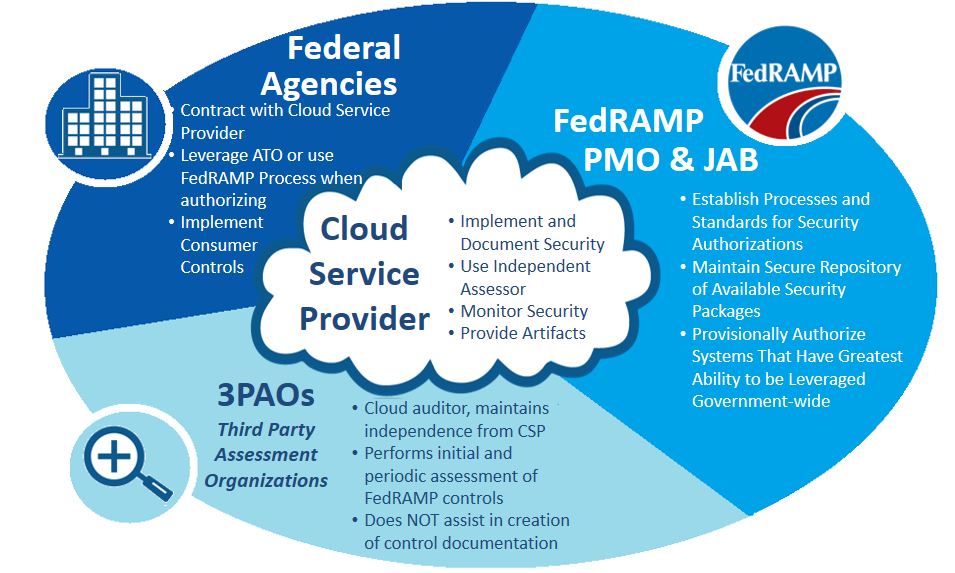
\includegraphics[width=\textwidth]{immagini/fedramp_actors.png}
}
\caption{Risk Management Framework, da \cite{} }\label{fig:fedrampactors}
\end{figure}



\subsubsection{Enti federali}
Agencies are responsible for
Ensuring all new cloud projects use the FedRAMP baseline controls and templates, as well as reviewing and granting authorizations
Ensuring existing cloud projects (implemented or in the acquisition process) meet FedRAMP requirements
Adding or modifying contractual provisions that require CSPs meet FedRAMP requirements
Updating OMB PortfolioStat data quarterly to identify use of CSPs and plans to meet FedRAMP requirements, and rationalize lack of compliance
Reviewing CSP documentation and test results prior to leveraging a JAB P-ATO or agency-issued ATO
Reviewing Plans of Action and Milestones (POAMs) for leveraged CSPs
Adding any agency-specific controls above the baseline
Submitting all documents for an agency-issued CSP authorization for leveraging by other agencies


\paragraph {Inventario}
Agencies should create an inventory of its respective cloud systems.  Not all agency systems are cloud systems, and agencies should determine which systems are cloud systems and which systems are traditional systems.  
FedRAMP recommends that agencies identify a liaison to centrally manage cloud systems and communicate FedRAMP requirements.  The liaison should be prepared to respond to agency queries and reporting requirements, and make agency-wide recommendations on FedRAMP.  The following information would be useful for the liaison to collect:
Name of cloud system
Description of what services the cloud system provides
Name and contact information of system owner
Date that the existing authorization was granted
Status of compliance with FedRAMP

\paragraph {Migrazione dei sistemi esistenti a FedRAMP}
Cloud systems implemented by agencies and CSPs prior to June 6, 2012 must have FedRAMP security controls in place by June 5, 2014.  Agencies should perform a gap analysis on their current cloud systems to determine which security controls are missing, and which security control parameters do not meet FedRAMP requirements.  
In some situations, an agency may have built their own cloud - either a private cloud or a cloud shared with another agency.  If an agency builds an in-house  cloud system, the agency must identify and implement missing security controls, and have the system tested by a third-party independent assessor.
If the cloud system was built by an external private sector CSP, the agency should inform the CSP that the system is not FedRAMP compliant, and advise the CSP that FedRAMP requirements should have been met by June 5, 2014.  If the CSP is not aware of FedRAMP requirements, the agency should direct the CSP to the FedRAMP website.  


\subsubsection{Organizzazioni di terze parti}

Title III, Section 3544, of the E-Government Act of 2002, dated December 17, 2002, requires agencies to conduct periodic assessments of the risk and magnitude of harm that could result from the unauthorized access, use, disclosure, disruption, modification, or destruction of information and information systems that support the operations and assets of the agency.  The term “system” includes Cloud Service Provider platforms and offerings.  Appendix III of Office of Management and Budget (OMB) Circular A-130, Management of Federal Information Resources, specifically requires federal agencies to:

To become an accredited 3PAO under FedRAMP, candidate third party assessors must submit application materials demonstrating that they meet both technical competence in security assessment of cloud systems and management requirements for organizations performing inspections. Prospective 3PAOs must have an operational Quality Management System in place at their organization and must demonstrate knowledge of standard conformity assessment processes.  
The 3PAO accreditation program ensures that approved 3PAOs consistently perform security assessments with an appropriate level of rigor and independence.  FedRAMP will only review security assessment packages from CSPs that have been assessed by an accredited 3PAO.  Furthermore, only CSPs that use an accredited 3PAO are eligible for a Joint Authorization Board (JAB) Provisional Authorization.
FedRAMP approved American Association for Laboratory Accreditation (A2LA) to accredit FedRAMP Third Party Assessment Organizations (3PAOs).  Using technical experts as assessors, the A2LA assessment process involves a rigorous evaluation of technical competence of the 3PAOs, as well as an assessment of their compliance to the general requirements of ISO/IEC 17020.  More information on working with A2LA and applying to become an accredited FedRAMP 3PAO can be found at http://a2la.org/fedramp.
FedRAMP retains governance and oversight of the 3PAO program, and maintains final approval authority for those 3PAO accredited by A2LA.


3.2. Security Testing
It is a goal of FedRAMP for all CSP systems to be assessed equally and according to the same security baseline controls appropriate for the designated sensitivity category.  In support of this goal, templates are provided to standardize the assessment process.  Templates designed for 3PAOs to complete or use are the Security Assessment Plan (SAP), Security Assessment Test Cases, and the Security Assessment Report (SAR).
3.2.1. Security Assessment Plan (SAP) 
The purpose of the SAP is to describe the security test plan.  The 3PAO must meet with the CSP to discuss the test engagement before developing the SAP, and again prior to finalizing the SAP.  If 3PAOs have any questions on security testing, they must contact the FedRAMP PMO ISSO.  The 3PAO must submit the final SAP to both the CSP and FedRAMP ISSO for approval prior to starting to test.  The ISSO will review the SAP and give the go ahead to start testing after obtaining approval from the JAB.  The SAP template is available on www.fedramp.gov. .  

3.2.2. Security Test Cases
The Security Assessment Test Cases are based on NIST SP 800-53A.  There are some FedRAMP test cases modified from NIST SP 800-53A due to the uniqueness of cloud implementations.  Therefore, it is important to use the test cases found on www.fedramp.gov. 
For any alternative implementations of controls as described in a CSPs SSP, the 3PAO must create alternative test cases that adequately test the effectiveness of the CSP’s control implementation and any risk associated with that implementation.
3.2.3. Security Assessment Report (SAR) 
The Security Assessment Report is the final report written by the 3PAO to detail the independent security assessment performed on the CSP candidate information system.  The FedRAMP PMO provides a Security Assessment Report template, and all 3PAOs are required to use this template to report their findings.  The SAR template is available on www.fedramp.gov. 
For JAB Provisional ATO’s, the 3PAO is expected to provide a high-level briefing to the FedRAMP PMO and JAB TRs. This brief will highlight findings, mitigations, and operational requirements, as well as identify any problems or areas of concern.  The FedRAMP ISSO coordinates with the 3PAO on the briefing. 
3.2.4. Running Scans
As part of security testing, automated scans are required.  On large implementations, a subset of all representative hosts and device types must be scanned using full authentication.  The advantage of running scans as fully authenticated privileged users is that the scanner can access the registry, file attributes, installed packages, and patch levels.  Account credentials for the authenticated scans must use login IDs and user roles that offer the greatest possible privileges for the scanned system (e.g. root, administrator).  
The use of non-authenticated scans can assist in vulnerability severity determinations and to prioritize remediation efforts since non-authenticated scan vulnerabilities are seen from the point of an attacker/intruder.  Non-authenticated scans can augment fully authenticated scans if the information from these scans helps to determine the risk exposure.  FedRAMP does not require non-authenticated scans.
3PAOs do not need to run source code scans.  However, if a CSP develops and uses original source code in their service offering, the CSP is required to perform source code scanning on the installed release and provide the source code analysis report to the 3PAO to satisfy control SA-11(1).  

Tip: 	An authenticated scan is sometimes referred to as credentialed scan or a host-based scan.

The 3PAO submits all scan results to the FedRAMP PMO ISSO at the same time the SAR is provided, and the 3PAO must be prepared to brief the results to the FedRAMP PMO and JAB representatives.  
A 3PAO scans CSP systems as part of the CSPs annual assessment.  The annual scan does not have to be performed by the same 3PAO that performed the previous scan(s).  


\subsubsection{Fornitori di servizi cloud}
A CSP can be a commercial or government entity that has a cloud offering or service.  The CSP is responsible for implementing FedRAMP security controls, hiring an independent third party assessor to perform initial and annual assessments, creating and maintaining its authorization, and complying with continuous monitoring requirements. Commercial CSPs must select an accredited 3PAO.    

1. A Cloud Service Provider can submit the appropriate documentation to the FedRAMP PMO and to the JAB which may grant a Provisional Authorization to Operate (P-ATO)
2. A Cloud Service Provider can submit the appropriate documentation to the FedRAMP PMO and to an agency which may grant an agency “Authorization to Operate” (ATO).  Using FedRAMP mechanisms, other agencies can then “leverage” this ATO for use in their agency, decreasing the time for approvals.
3. A Cloud Service Provider can use the “CSP supplied” path by submitting the appropriate documentation to the FedRAMP PMO.  While this does not grant the CSP a P-ATO or an agency ATO, it decreases the time for approvals because documentation and testing (by a 3PAO) are complete and available for agency review.




A cloud system is compliant with FedRAMP if it meets the following requirements:
The system security package has been created using the required FedRAMP templates
The system meets the FedRAMP security control requirements
The system has been assessed by an independent assessor
A Provisional Authorization, and/or an Agency ATO, has been granted for the system
An authorization letter for the system is on file with the FedRAMP Program Management Office (PMO)



Cloud service providers (CSPs) initiate participation in FedRAMP by submitting a FedRAMP Initiation Request form.  This is a web based form found on the FedRAMP website.  This form advises the FedRAMP PMO, and the JAB of the intent to obtain a FedRAMP Provisional Authorization.  
On the FedRAMP Initiation Request form, a CSP provides a categorization of its system and indicate the information types based upon NIST SP 800-60 V2 guidelines.  CSPs must use the data type sensitivity categorization to select which control baseline to implement – Low or Moderate.  (High sensitivity categorizations are currently not part of the FedRAMP program.)  The FedRAMP PMO contacts the CSP to schedule a conference call to discuss CSP readiness to begin the process to achieve Provisional Authorization.
At this time, the CSP must research and hire a 3PAO.  FedRAMP accredited 3PAOs are listed on the FedRAMP website.  

5.3. After Acceptance into the FedRAMP Program
After acceptance into the FedRAMP JAB Provisional Authorization process, there are certain documents requiring submission.  The FedRAMP PMO created templates for documents that the CSP must edit and modify based on the security controls implemented in its system.  All templates are available on the FedRAMP website.  Guidance on how to fill out the various templates and develop the required documents are described in the sections that follow.  




\section{FedRAMP readiness}

In prior cloud FISMA compliance projects, certain controls proved to be challenging for CSPs to meet.  Before a CSP decides to initiate a request to participate in FedRAMP, it must review the checklist in Table 5-1 to ensure ability to meet the requirements.  CSPs must consult with legal and technical staff (e.g.  systems administrators, database administrators, network engineers) to determine whether appropriate controls are in place and manageable.


\section{Controlli di sicurezza per la conformità}
.\\\newpage
.\\\newpage
.\\\newpage
.\\\newpage
\section{FedRAMP in Amazon AWS}
.\\\newpage
.\\\newpage
\end{document}
